\section{Sequential-COGITAO}\label{appendix:sequential_COGITAO}

\begin{figure}[!htbp]
    \centering
    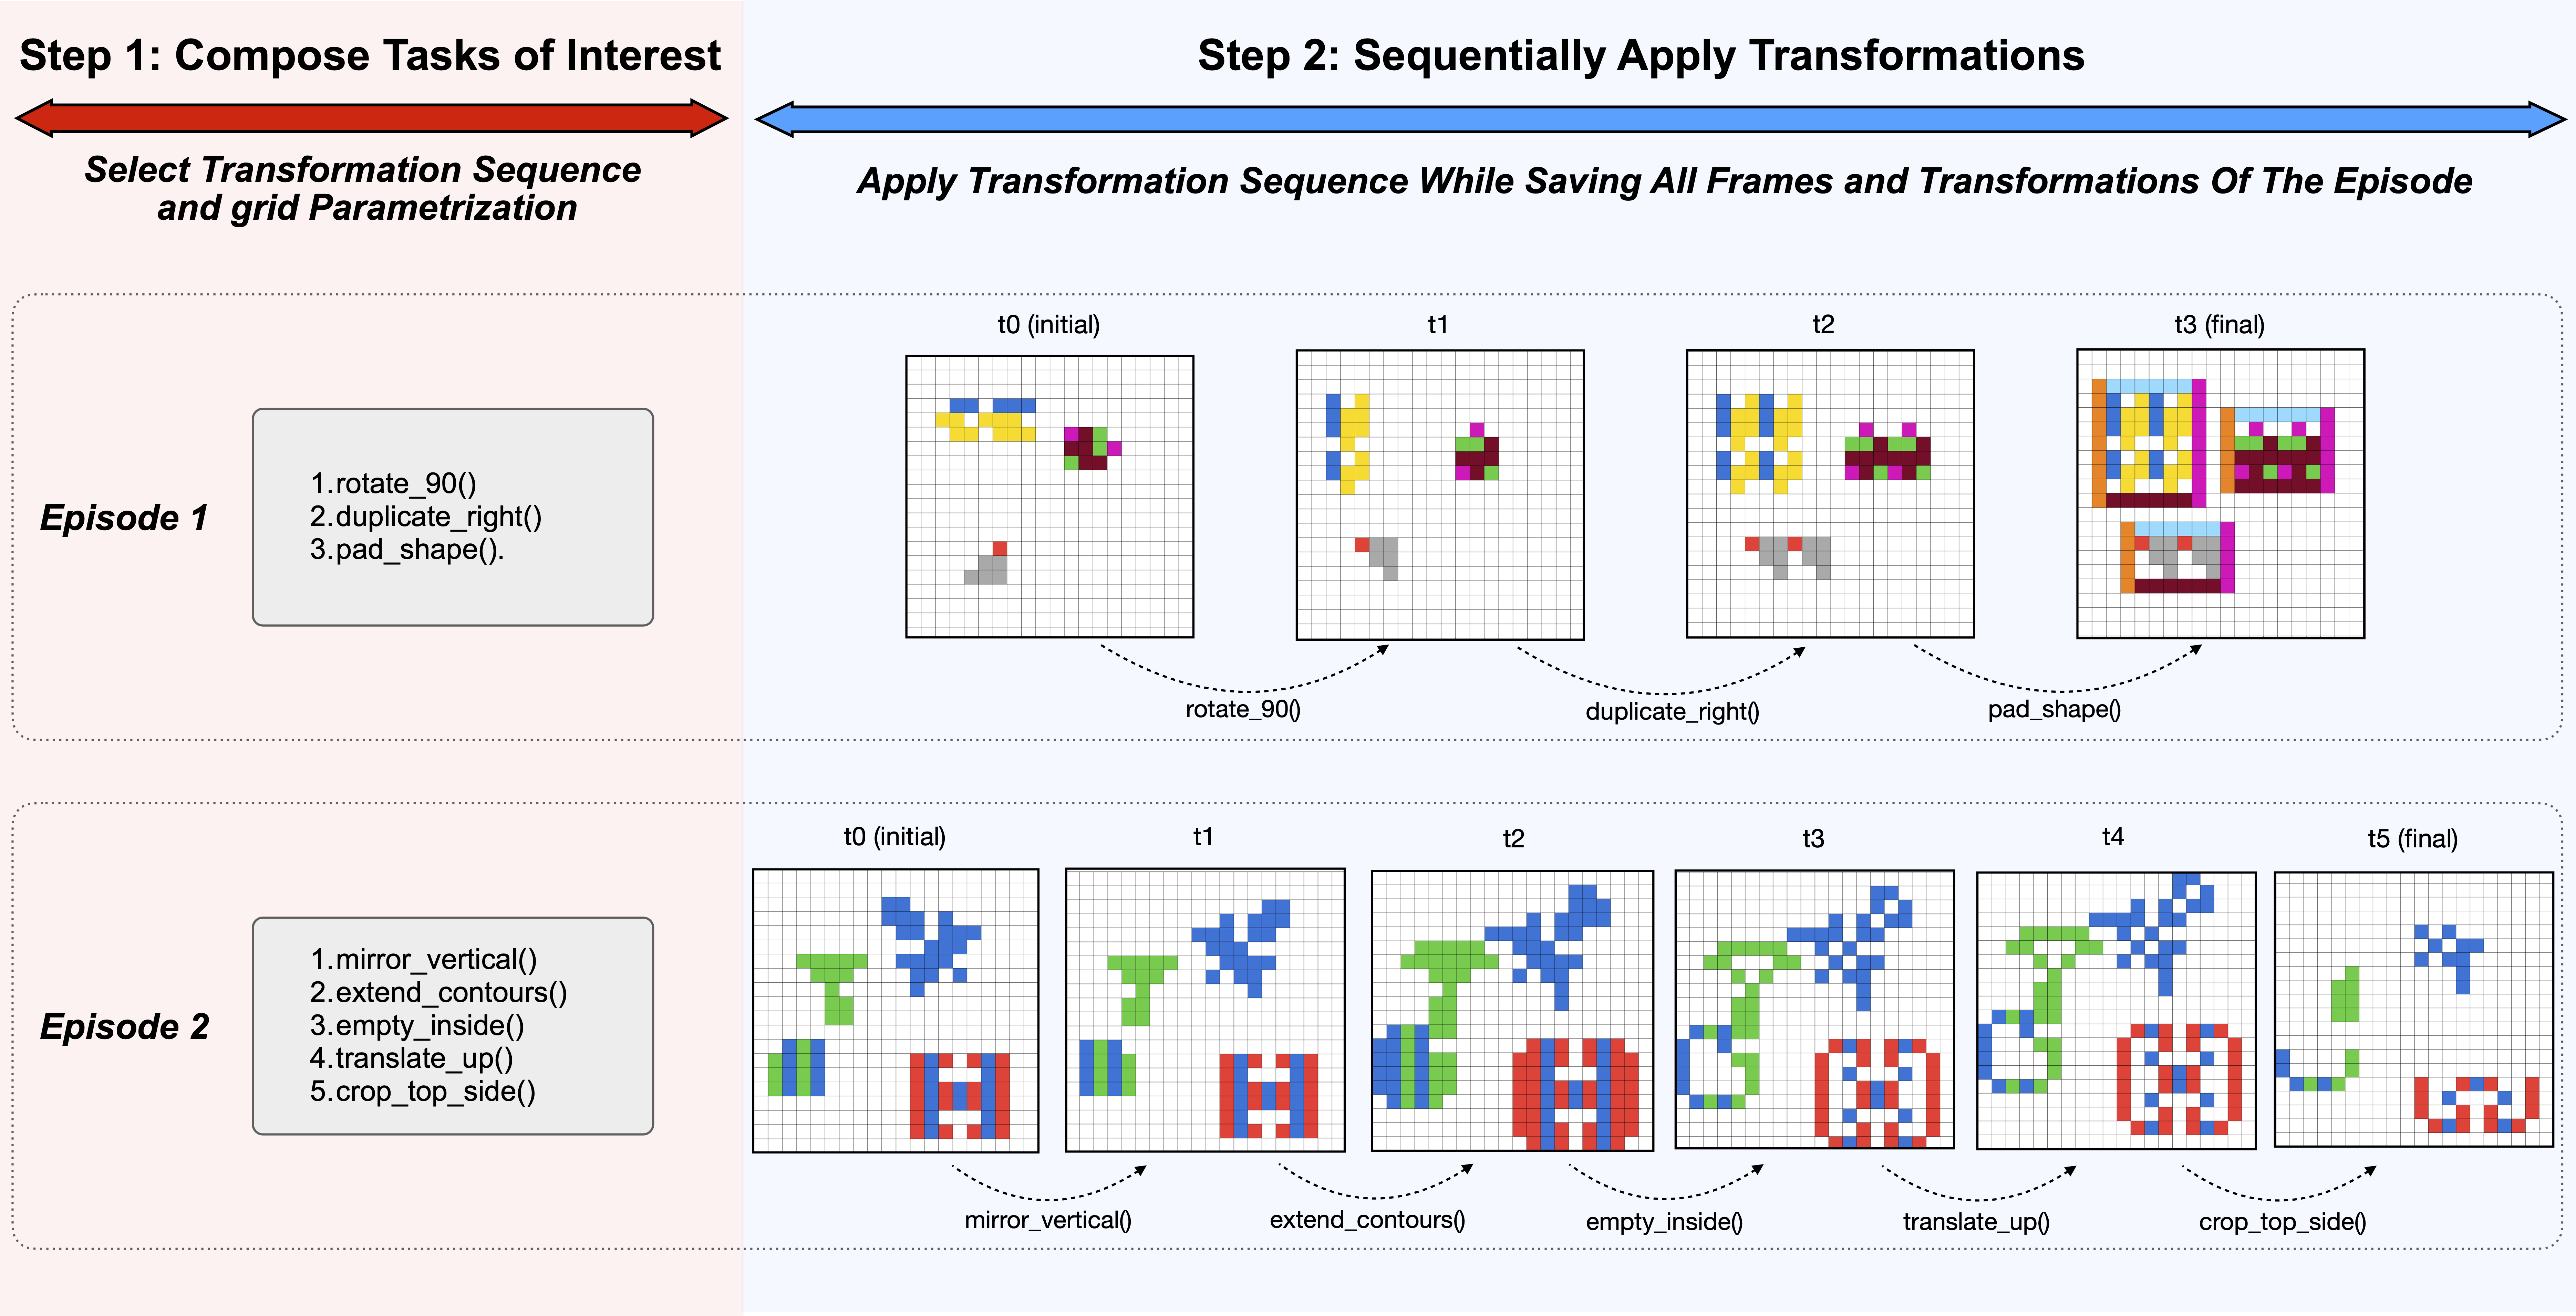
\includegraphics[width=1\columnwidth]{Figures/sequence_cogitao_figure.png}
    \caption{Overview of Sequential-COGITAO.  Episodes of are generated from an initially sampled transformation sequence and grid parametrization. Each individual frame is saved, along with its corresponding transformations. We note that transitions for each individual objects are also available, but not shown here for visualization constraints.}
    \label{fig:sequential_COGITAO}
\end{figure}

Standard COGITAO tasks present a single input grid and expect a model to generate the final output after a composed transformation sequence. Sequential COGITAO extends this by exposing every intermediate state in the transformation chain. Instead of training solely on start–end pairs, models must either predict each intermediate grid or reason over an explicit temporal trajectory of transformations. This is particularly relevant for World Model research \cite{ha2018world}, where applying action to objects while preserving the environment is of particular importance \cite{hafner2023masteringDREAMER, bruce2024GENIE, ferraro2025FOCUS}. Both \textit{CompGen} and \textit{EnvGen} methodologies can seamlessly be applied to Sequential-COGITAO (also in a RGB rendering; see \ref{appendix:rgb_cogitao}), enabling targeted and compositionality-focused research on perception and interaction tasks---a needed addition to the field. 
